% PCCSL 507 Machine Learning Lab - Experiment 8 (NumPy only)
\documentclass[11pt,twoside]{article}

\usepackage[paper=letterpaper,top=0.7in,bottom=0.63in,left=0.75in,right=0.75in,headheight=24pt,headsep=0.14in,footskip=0.38in]{geometry}

\usepackage[T1]{fontenc}
\usepackage{mathptmx} % Times clone
\usepackage{xcolor}
\definecolor{primary}{HTML}{1F3864}
\usepackage{fancyhdr}
\usepackage{array}
\usepackage{colortbl}
\usepackage{parskip}
\setlength{\parindent}{0pt}
\setlength{\parskip}{4pt}
\setlength{\abovedisplayskip}{4pt}
\setlength{\belowdisplayskip}{4pt}
\setlength{\abovedisplayshortskip}{2pt}
\setlength{\belowdisplayshortskip}{2pt}
\usepackage{graphicx}
\usepackage{amsmath}
\usepackage{listings}
\lstset{basicstyle=\footnotesize\ttfamily, breaklines=true, frame=single, showstringspaces=false}

\pagestyle{fancy}
\fancyhf{}
\fancyhead[C]{\textcolor{primary}{\textbf{\small PCCSL 507 Machine Learning Laboratory Record}}}
\renewcommand{\headrulewidth}{0.75pt}
\renewcommand{\headrule}{\hbox to\headwidth{\color{primary}\leaders\hrule height \headrulewidth\hfill}}
\fancyfoot[C]{\footnotesize DEPARTMENT OF CSE \hfill CAPE COLLEGE OF ENGINEERING ALAPPUZHA \hfill Page No. \thepage}
\renewcommand{\footrulewidth}{0pt}

\newcommand{\expheading}[1]{{\fontsize{14}{17}\selectfont\textbf{#1}\par}}
\newcommand{\fullrule}{\noindent\rule{\textwidth}{0.6pt}\par}

\begin{document}
\sloppy

% Sheet-local tightening so it fits one right-side page
{\setlength{\parskip}{1pt}\setlength{\abovedisplayskip}{2pt}\setlength{\belowdisplayskip}{2pt}
\begin{center}
\expheading{EXPERIMENT NO. 8}
\end{center}
\vspace{2pt}

\noindent\textbf{Date:} \underline{\hspace{2.6cm}}\par
\vspace{6pt}

\expheading{TITLE}
\vspace{4pt}
\noindent Ridge and Lasso Regression on Diabetes Dataset\par
\vspace{4pt}

\expheading{AIM}
\vspace{4pt}
\noindent To fit ordinary, Ridge and Lasso models on diabetes data, pick penalties by 5-fold cross-validation, and compare test MSE and $R^2$. \par
\vspace{4pt}

\expheading{OBJECTIVE}
\vspace{2pt}
\fullrule
\vspace{4pt}
\noindent To implement Ridge and Lasso regression on the Diabetes dataset, tune penalties by cross-validation, and compare with standard linear regression using MSE and R-squared. \par
\vspace{4pt}

\expheading{THEORY}
\vspace{4pt}
Standard linear regression (normal equation):
\[\theta=(X^TX)^{-1}X^Ty\]
Ridge objective and closed form ($\lambda$ unpenalized intercept via centering):
\[J=\|y-Xw\|^2+\lambda\|w\|^2\qquad w=(X^TX+\lambda I)^{-1}X^Ty\]
Lasso objective and coordinate-descent update (soft thresholding):
\[J=\|y-Xw\|^2+\lambda\|w\|_1\qquad w_j=\frac{S(\rho_j,\lambda)}{z_j},\;S(\rho,\lambda)=\mathrm{sign}(\rho)\max(|\rho|-\lambda,0)\]
Cross-validation picks the $\lambda$ with lowest mean validation MSE; report test MSE and $R^2$.
\vspace{4pt}

\expheading{PROCEDURE}
\vspace{4pt}
\noindent 1. Load diabetes data (442$\times$10); 80/20 split (seed 42); standardize $X$, center $y$ (intercept unpenalized).\par
\noindent 2. Fit ordinary least squares by normal equation; record test MSE and $R^2$.\par
\noindent 3. Fit Ridge in closed form over a $\lambda$ grid; pick best $\lambda$ by 5-fold cross-validation.\par
\noindent 4. Fit Lasso by coordinate descent over an $\alpha$ grid; pick best $\alpha$ by 5-fold cross-validation.\par
\noindent 5. Compare test MSE, $R^2$ and sparsity; plot CV curves. \par
\vspace{4pt}

\expheading{DATASET DESCRIPTION}
\vspace{4pt}
\noindent Dataset Name: Diabetes (diabetes.tab.txt)\par
\noindent Source: 442 patients; 10 baseline variables (age, sex, bmi, bp, s1--s6)\par
\noindent Number of Samples: 353 train / 89 test \hspace{0.3cm} Number of Features: 10\par
\noindent Target / Class: Disease progression (continuous)\par
\noindent Description: 80/20 split, seed 42; $X$ standardized, $y$ centered. \par
\vspace{4pt}
} % end sheet-local tightening

\newpage
\expheading{PROGRAM}
\vspace{6pt}

\begin{lstlisting}
import numpy as np
import matplotlib
matplotlib.use("Agg")
import matplotlib.pyplot as plt
CSV = "diabetes.tab.txt"
data = np.loadtxt(CSV, delimiter="\t", skiprows=1)
X_all, y_all = data[:, :10], data[:, 10]
print("Dataset:", X_all.shape)
rng = np.random.default_rng(42)
idx = np.arange(len(X_all))
rng.shuffle(idx)
ntr = int(0.8 * len(idx))
tri, tei = idx[:ntr], idx[ntr:]
Xtr_raw, Xte_raw, ytr, yte = X_all[tri], X_all[tei], y_all[tri], y_all[tei]
print("Train:", len(tri), " Test:", len(tei))
mu, sg = Xtr_raw.mean(0), Xtr_raw.std(0); yb = ytr.mean()
Xtr, Xte = (Xtr_raw - mu) / sg, (Xte_raw - mu) / sg; ytrc = ytr - yb
def ridge_fit(X, y, lam):
    p = X.shape[1]
    return np.linalg.inv(X.T @ X + lam * np.eye(p)) @ X.T @ y
def lasso_fit(X, y, lam, iters=300):
    n, p = X.shape
    w = np.zeros(p)
    for _ in range(iters):
        for j in range(p):
            rho = X[:, j] @ (y - X @ w + w[j] * X[:, j]) / n
            z = (X[:, j] ** 2).mean()
            w[j] = np.sign(rho) * max(abs(rho) - lam, 0.0) / z
    return w
def mse(a, b):
    return float(((a - b) ** 2).mean())
def r2(ys, p):
    return float(1 - ((ys - p) ** 2).sum() / ((ys - ys.mean()) ** 2).sum())
w_ols = np.linalg.inv(Xtr.T @ Xtr) @ Xtr.T @ ytrc
p_ols = Xte @ w_ols + yb
print(f"OLS: MSE={mse(yte, p_ols):.4f} R2={r2(yte, p_ols):.4f}")
folds = np.array_split(rng.permutation(ntr), 5)
def cv_score(lam, lasso):
    e = 0.0
    for k in range(5):
        va = folds[k]
        tr = np.concatenate([folds[j] for j in range(5) if j != k])
        w = (lasso_fit if lasso else ridge_fit)(Xtr[tr], ytrc[tr], lam)
        e += ((ytr[va] - (Xtr[va] @ w + yb)) ** 2).mean()
    return e / 5
rlams = [0.1, 1.0, 10.0, 100.0]; llams = [0.1, 0.5, 1.0, 5.0]
rms = [cv_score(l, False) for l in rlams]; lms = [cv_score(l, True) for l in llams]
bl, ba = rlams[int(np.argmin(rms))], llams[int(np.argmin(lms))]
print(f"Best: Ridge lam={bl}, Lasso alpha={ba}")
w_r = ridge_fit(Xtr, ytrc, bl); w_l = lasso_fit(Xtr, ytrc, ba)
p_r, p_l = Xte @ w_r + yb, Xte @ w_l + yb
print(f"Ridge: MSE={mse(yte, p_r):.4f} R2={r2(yte, p_r):.4f}")
print(f"Lasso: MSE={mse(yte, p_l):.4f} R2={r2(yte, p_l):.4f}")
print("Nonzero Ridge/Lasso:", (w_r != 0).sum(), (w_l != 0).sum())
plt.figure(figsize=(7, 4.5))
plt.semilogx(rlams, rms, marker="o", linewidth=2, label="Ridge CV")
plt.semilogx(llams, lms, marker="s", linewidth=2, label="Lasso CV")
plt.xlabel("Lambda"); plt.ylabel("5-fold CV MSE"); plt.grid(True)
plt.title("Cross-Validation: Ridge vs Lasso"); plt.legend(); plt.tight_layout()
plt.savefig("exp8_cv.png", dpi=150)
\end{lstlisting}

\newpage
\expheading{OUTPUT}
\vspace{2pt}
\noindent\rule{\textwidth}{0.5pt}\par
\vspace{4pt}
\begin{verbatim}
Dataset: (442, 10)
Train: 353  Test: 89
OLS: MSE=2594.6297 R2=0.5927
Best: Ridge lam=1.0, Lasso alpha=0.5
Ridge: MSE=2596.3521 R2=0.5924
Lasso: MSE=2623.3691 R2=0.5882
Nonzero Ridge/Lasso: 10 8
\end{verbatim}
\vspace{4pt}

\begin{center}
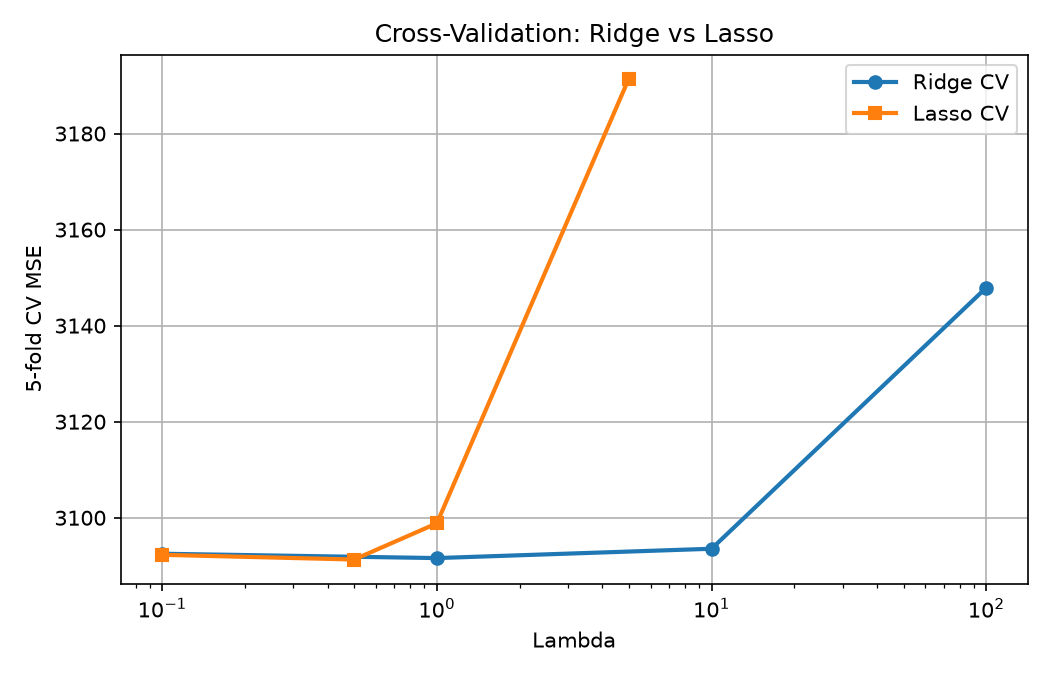
\includegraphics[width=0.78\textwidth]{exp8_cv.png}\par
\small Fig. 1: 5-fold CV MSE vs penalty (best: Ridge $\lambda=1$, Lasso $\alpha=0.5$).\par
\end{center}
\vspace{4pt}

\expheading{RESULT}
\vspace{4pt}
{\fontsize{12}{15}\selectfont
The above program was implemented and executed successfully using Python, and the corresponding output was obtained and verified. The results of the \textbf{Ridge and Lasso regression} were analyzed and found to be satisfactory, thereby achieving the desired objective of the experiment.\par
}

\vspace{12pt}

\noindent\textbf{Faculty Signature:} \underline{\hspace{3.6cm}} \hfill \textbf{Date:} \underline{\hspace{2.8cm}}\par

\end{document}
